% Author: João Vitor Silva Mendes
% Email: vitormendesrb@gmail.com or vitor.mendes@ieee.org
% GitHub: github.com/vitorsmends

\documentclass{cubeamer}

\title{Title}
\subtitle{Subtitle}
\author[Nome e sobrenome]{Nome e sobrenome.}
\date{\today} % or whatever the date you are presenting in is
\institute[SENAI CIMATEC]{SENAI CIMATEC - IEEE ROBOTICS AND AUTOMATION SOCIETY}
% \copyrightnotice{Published by the American Institute of Aeronautics and Astronautics, Inc., with permission}
\usepackage{ragged2e}
\begin{document}

\maketitle

\cutoc

\section{Introdução}

\begin{frame}{RAS CIMATEC}
    \begin{columns}
        \begin{column}{0.4\textwidth}
            \begin{itemize}
                \item Topics
                \item Topics
                \item Topics
            \end{itemize}
        \end{column}

        \begin{column}{0.6\textwidth}
            \begin{figure}
                \centering
                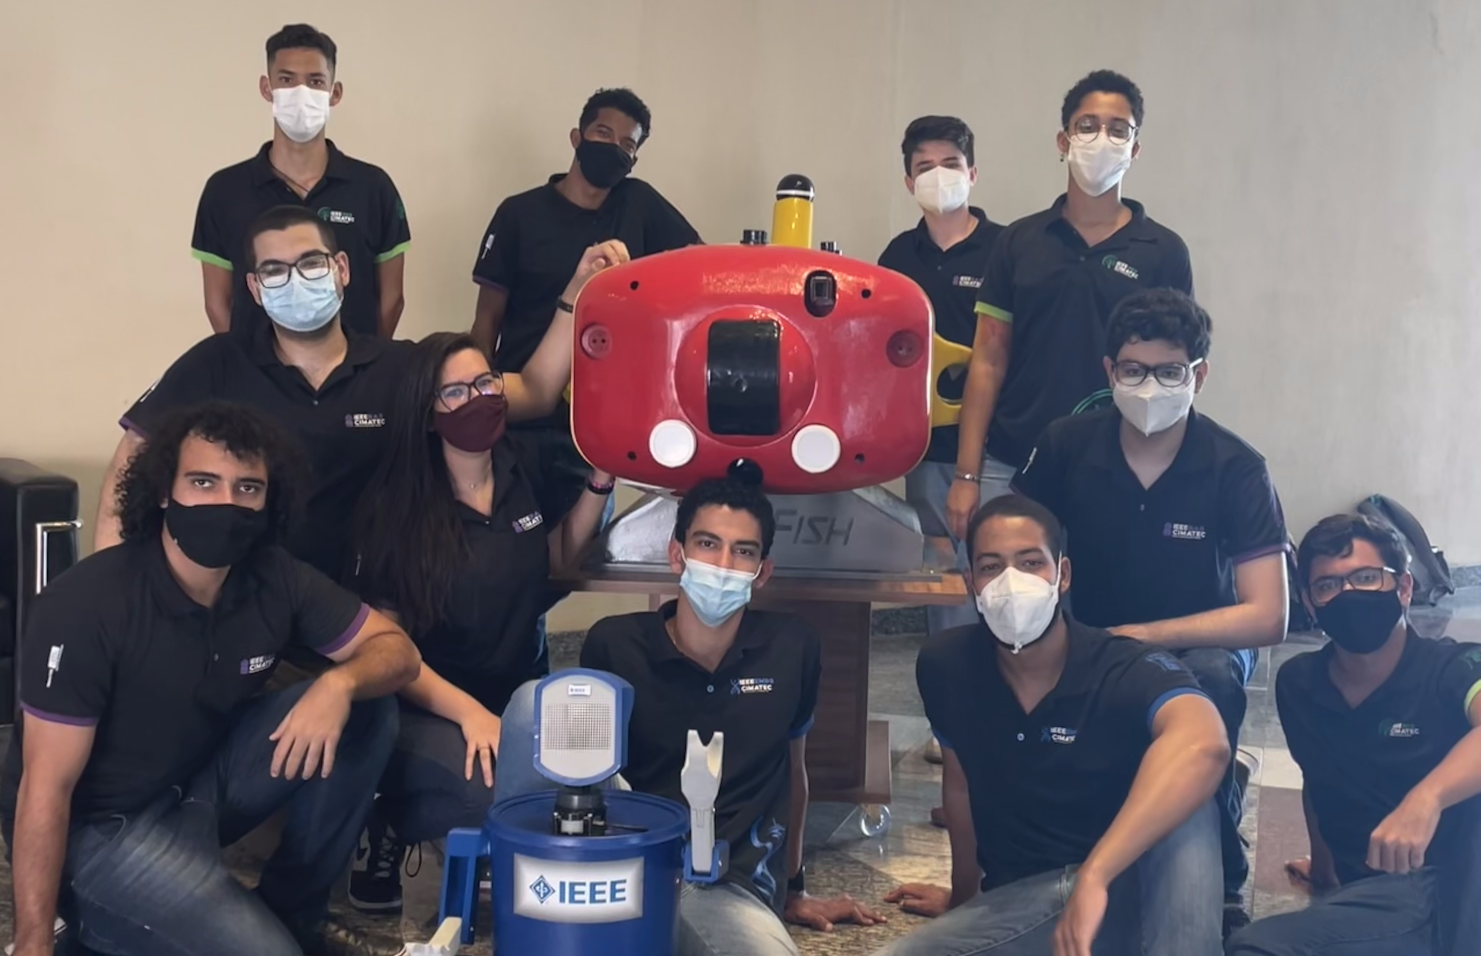
\includegraphics[height = 0.6\textheight]{img/team2.png}
                \caption{IEEE CIMATEC members \textit{Source et al.}}
            \end{figure}
        \end{column}

    \end{columns}
\end{frame}

\begin{frame}{Author}
    \begin{columns}
        \centering
        \begin{column}{0.3\textwidth}
            \begin{figure}
                \centering
                
\includegraphics[height = 0.5\textheight]{img/mediador.png}
                \caption[]{Vítor Mendes}
            \end{figure}
        \end{column}
        \centering
        \begin{column}{0.5\textwidth}
            \footnotesize
            \justifying
            You can introduce yourself here.

        \end{column}
    \end{columns}
\end{frame}

\begin{frame}{Two columns}
    \begin{columns}
        \centering
        \begin{column}{0.4\textwidth}
            \textbf{Title} \\
            \small
            Text here.

        \end{column}
        \begin{column}{0.5\textwidth}
            \textbf{Title} \\
            \small
            Text here.
        \end{column}
    \end{columns}
\end{frame}



\begin{frame}{Arduino}

    \begin{figure}
        \centering
        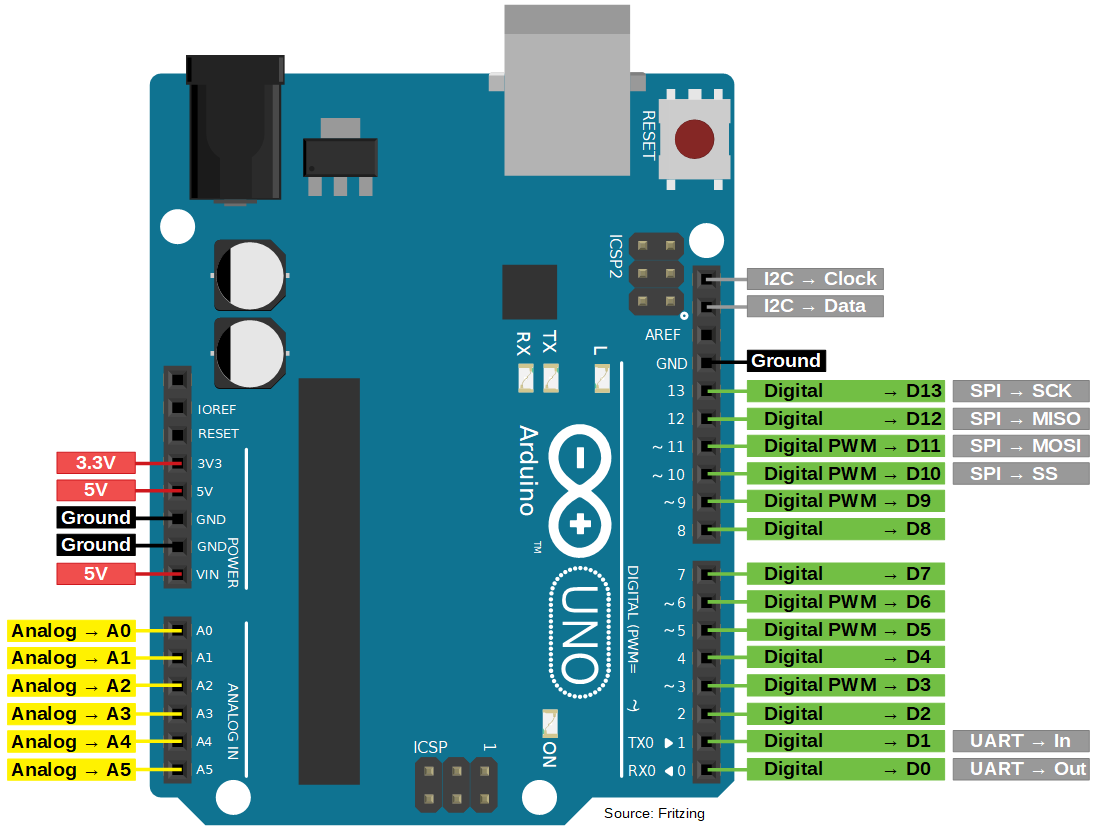
\includegraphics[height = 0.5\textheight]{img/uno.png}
        \caption{Maybe just a image.}
    \end{figure}

\end{frame}

\section{What about questions?}

\begin{frame}{Make your presentation interactive}
    \begin{cublock}[What about a question to the audience?]
        \begin{overlayarea}{\textwidth}{\baselineskip}
            \only<2->{Followed by the answer.}
        \end{overlayarea}
    \end{cublock}
\end{frame}

% Q&A
\begin{frame}[standout]
    \Huge\textsc{Questions?}
    
    \vfill
    
    \LARGE\textsc{vitor.mendes@ieee.org}
\end{frame}

\appendix

\begin{frame}{Backup slides go here}
    
\end{frame}

\end{document}
